%Please use LuaLaTeX or XeLaTeX
\documentclass[11pt,aspectratio=169,reqno]{beamer}

\title{Math meets Biology}
\date[28.03.2023]{28.03.2023}
\author{Mario Kunz, Xaver Hanushevsky}
\institute{D-BIOL}

\usetheme{eth}

\colorlet{titlefgcolor}{ETHBlue}
\colorlet{accentcolor}{ETHRed}

\newcommand{\highlightpause}{\addtocounter{beamerpauses}{-1}\pause\color<+>{ETHPurple}}

\begin{document}

\titleframe

\begin{frame}[fragile]{Intro}
    Etwas Kreatives einfallen lassen für hier
\end{frame}

\begin{frame}{Was ist Rückkopplung...}
Positiv und negative Rückkopplung mit Bild erklären
Erwartungen an unsere Lösungen (Positiv => $\infty$)
\end{frame}

\begin{frame}{Repression des lac-operons}
@Mario Bild

Zeichnung des Schemas, vorerst aber ohne Beachtung der Bindung von Lactose/Allolactose
\end{frame}

\begin{frame}{Genregulation über DNA-bindendes Protein}
    Jetzt nochmal mit negativer Autoregulation @mario

    \begin{figure}
        \centering
        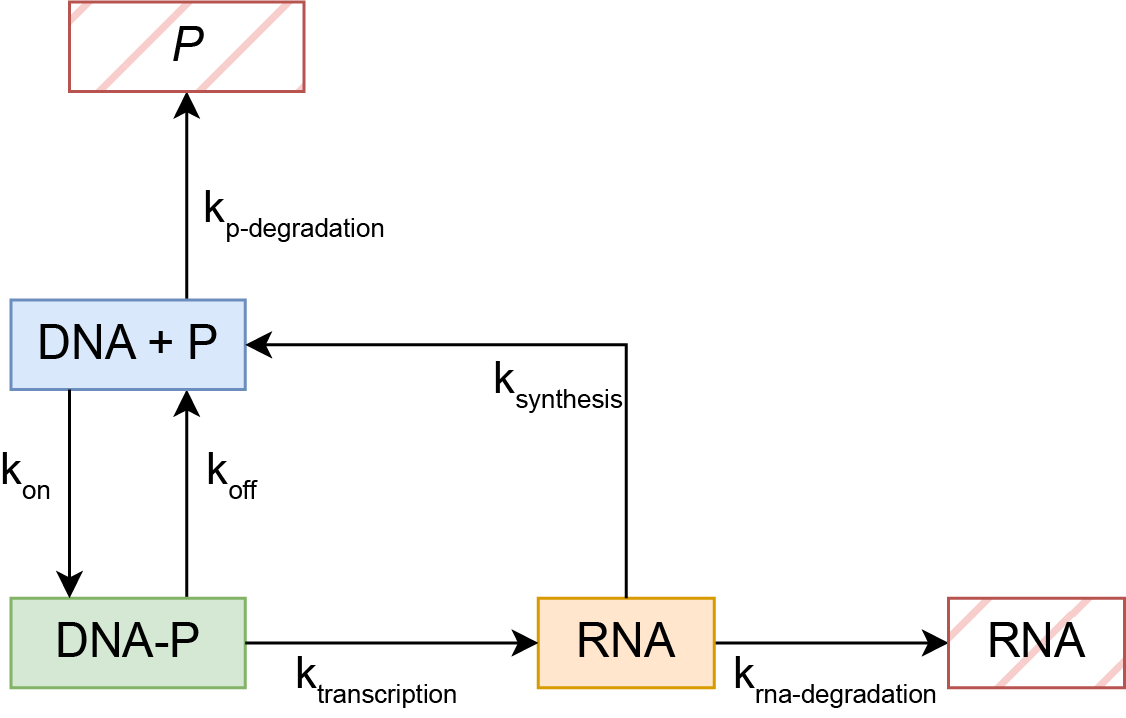
\includegraphics[width=.6\textwidth]{images/gene_regulation_overview.png}
        \label{fig:my_label}
    \end{figure}
\end{frame}

\begin{frame}{Gleichgewicht zwischen gebundener und freier DNA}
    \begin{tikzpicture}[remember picture,overlay]
        \node[xshift=-2cm,yshift=-2cm] at (current page.north east) {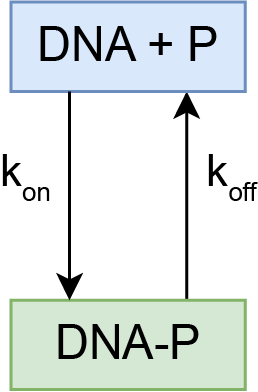
\includegraphics[width=2cm]{images/DNA-binding_equilibrium.png}};
    \end{tikzpicture}

    \emph{Annahmen konkretisieren/genauer erklären}
    Nur ungebundene DNA führt zu Transkription

    \begin{itemize}
        \item $v_\text{on}=k_\text{on}\cdot [\text{DNA}]\cdot [\text{P}]$
        \item $v_\text{off}=k_\text{off}\cdot [\text{DNA-P}]$\pause
        \item Im Gleichgewicht gilt 
        \begin{itemize}
            \item $v_\text{on}=v_\text{off}$\\[8pt]
            \item $\dfrac{d[\text{DNA}]}{dt}=\dfrac{d[\text{DNA-P}]}{dt}=0$\\[8pt]
            \item[$\Rightarrow$] $k_\text{on}\cdot [\text{DNA}]\cdot [\text{P}]=k_\text{off}\cdot [\text{DNA-P}]$
        \end{itemize}
    \end{itemize}
\end{frame}

\begin{frame}{Gleichgewicht zwischen gebundener und freier DNA}    
    \begin{columns}[T]
    \column{.3\textwidth}
    \centering
    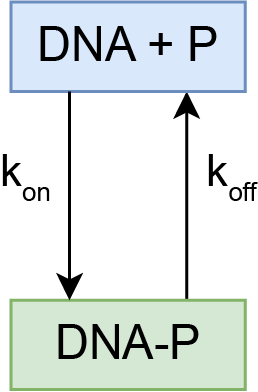
\includegraphics[width=2cm]{images/DNA-binding_equilibrium.png}
    \column{.3\textwidth}\highlightpause
    \[K=\frac{k_\text{off}}{k_\text{on}}=\frac{[\text{DNA}]\cdot [\text{P}]}{[\text{DNA-P}]}\]
    \column{.3\textwidth}\highlightpause
        \[[\text{DNA$_\text{Total}$}]=[\text{DNA}]+[\text{DNA-P}]\]\\[-1em]
        \[[\text{DNA}]=[\text{DNA$_\text{Total}$}]-[\text{DNA-P}]\]
    \end{columns}\\[-4em]\highlightpause
    \parbox{\textwidth}{
    \[\Downarrow\]
    \[K=\frac{([\text{DNA$_\text{Total}$}]-[\text{DNA-P}])\cdot [\text{P}]}{[\text{DNA-P}]}\]\\\highlightpause
    \[K\cdot[\text{DNA-P}]=[\text{DNA$_\text{Total}$}]\cdot [\text{P}]-[\text{DNA-P}]\cdot [\text{P}]\]\highlightpause
    \[[\text{DNA-P}]\cdot(K+[\text{P}])=[\text{DNA$_\text{Total}$}]\cdot [\text{P}]\]\\\highlightpause
    \[[\text{DNA-P}]=\frac{[\text{DNA$_\text{Total}$}]\cdot [\text{P}]}{(K+[\text{P}])}\]
    }
\end{frame}

\begin{frame}{Vergleich mit Enzymkinetik, FiB 1}
    @Mario

    \begin{columns}
        \column{.5\textwidth}
        \[[\text{DNA-P}]=[\text{DNA$_\text{Total}$}]\cdot\color{ETHPurple}\frac{[\text{P}]}{(K+[\text{P}])}\]
        \column{.5\textwidth}
        a
    \end{columns}
\end{frame}

\begin{frame}{Von Besetzungsgrad zum Nichtbesetzungsgrad}
@Mario
\end{frame}

\begin{frame}{Mathematische Modellierung}
@Xaver
\emph{Mit Overview neuen Kontext einleiten}
\end{frame}

\begin{frame}{Mathematische Modellierung}
\begin{equation}
    \frac{d[\text{RNA}]}{dt}=[\text{RNA}]_{\text{Synthese}}-[\text{RNA}]_{\text{Abbau}}
\end{equation}
\\[12pt]
\begin{equation}
    \frac{d[P]}{dt}=[P]_{\text{Synthese}}-[P]_{\text{Abbau}}
\end{equation}
\end{frame}

\begin{frame}[t]{Mathematische Modellierung mRNA}
    \begin{tabular}{l l}
        $\dfrac{d[\text{RNA}]}{dt} =[\text{RNA}]_{\text{Synthese}}-\textcolor{red}{[\text{RNA}]_{\text{Abbau}}}$ &  \\
    \end{tabular}
    \begin{equation}\notag
        [\text{RNA}]_{\text{Abbau}}=[\text{RNA}] \cdot k_{dr}
    \end{equation}
\end{frame}

\begin{frame}[t]{Mathematische Modellierung mRNA}
w2    \begin{tabular}{l l}
        $\dfrac{d[\text{RNA}]}{dt} =[\text{RNA}]_{\text{Synthese}}-{[\text{RNA}]_{\text{Abbau}}}$ &  \\
    \end{tabular}
    \begin{equation}\notag
        [\text{RNA}]_{\text{Abbau}}=[\text{RNA}] \cdot k_{dr}
    \end{equation}
    \\[16pt]
    \begin{tabular}{l l}
        $\dfrac{d[\text{RNA}]}{dt} =\textcolor{ETHRed}{[\text{RNA}]_{\text{Synthese}}}-{[\text{RNA}]_{\text{Abbau}}}$ &  \\
    \end{tabular}
    \begin{equation}\notag
        [\text{RNA}]_{\text{Synthese}}=v_{\text{max}}\cdot\frac{K}{K+[P]}
    \end{equation}
\end{frame}

\begin{frame}[t]{Mathematische Modellierung mRNA}
    \begin{tabular}{l l}
        $\dfrac{d[\text{RNA}]}{dt} =[\text{RNA}]_{\text{Synthese}}-\textcolor{ETHBlue}{[\text{RNA}]_{\text{Abbau}}}$ &  \\
    \end{tabular}
    \begin{equation}\notag
        \textcolor{ETHBlue}{
        [\text{RNA}]_{\text{Abbau}}}=[\text{RNA}] \cdot k_{dr}
    \end{equation}
    \\[16pt]
    \begin{tabular}{l l}
        $\dfrac{d[\text{RNA}]}{dt} =\textcolor{ETHPurple}{[\text{RNA}]_{\text{Synthese}}}-[\text{RNA}]_{\text{Abbau}}$ &  \\
    \end{tabular}
    \begin{equation}\notag
    \textcolor{ETHPurple}{\text{RNA}_{\text{Synthese}}}=v_{\text{max}}\cdot\frac{K}{K+[P]}
    \end{equation}
    \\[16pt]
    \begin{equation}\tag{1}
        \frac{d[\text{RNA}]}{dt}=v_{\text{max}}\cdot\frac{K}{K+[P]}-[\text{RNA}] \cdot k_{dr}
    \end{equation}
\end{frame}

\begin{frame}[t]{Mathematische Modellierung Protein}
    \begin{tabular}{l l}
        $\dfrac{d[P]}{dt} =[P]_{\text{Synthese}}-{[P]_{\text{Abbau}}}$ &  \\
    \end{tabular}
    \begin{equation}\notag
        [P]_{\text{Abbau}}=[P] \cdot k_{dr}
    \end{equation}
    \\[16pt]
    \begin{equation}\notag
        [P]_{\text{Synthese}}=k_{s}\cdot[\text{RNA}]
    \end{equation}
    \\[16pt]
    \begin{equation}\tag{2}
        \frac{d[P]}{dt}=k_{s}\cdot[\text{RNA}]-[P] \cdot k_{dr}
    \end{equation}
\end{frame}

\begin{frame}{Mathematische Modellierung}

\begin{align}
    \frac{d[\text{RNA}]}{dt}&=v_{\text{max}}\cdot\frac{K}{K+[P]}-[\text{RNA}] \cdot k_{dr} \tag{1} \\[16pt]
    \frac{d[P]}{dt}&=k_{s}\cdot[\text{RNA}]-[P] \cdot k_{dr} \tag{2}
\end{align}

\end{frame}

\begin{frame}{Stationäre Lösung mRNA herleiten}
@Xaver
\end{frame}

\begin{frame}{Konstanten}
    @Xaver
    \emph{Stationäre Lösung numerisch lösen}
\end{frame}

\begin{frame}{Stationäre Lösung Protein}
@Xaver
Nur eines der beiden herleiten
\end{frame}

\begin{frame}{Numerische Lösung mit Matlab}
@Mario
\end{frame}

\begin{frame}{Biologische Bedeutung}
\end{frame}

\begin{frame}{Vergleich mit positiver Rückkopplung}
@Mario matlab Lösung zeigen
\end{frame}

\begin{frame}{Vereinfachungen}
    \begin{itemize}
        \item 
    \end{itemize}
\end{frame}

\end{document}